\documentclass[sigplan,10pt,screen]{acmart}
\renewcommand\footnotetextcopyrightpermission[1]{}
\pagestyle{plain}

\usepackage{datetime}
\usepackage{url}
\usepackage{hyperref}
\usepackage{xspace}
\usepackage{amssymb}% http://ctan.org/pkg/amssymb
\usepackage{pifont}% http://ctan.org/pkg/pifont
\usepackage{todonotes}
\usepackage{cleveref}
\usepackage{tabularx}
\usepackage{booktabs}
\usepackage{multirow}
\usepackage{algorithm}
\usepackage[noend]{algpseudocode}
\usepackage{subcaption}

 \aboverulesep=0ex
 \belowrulesep=0ex
 
\crefformat{section}{\S#2#1#3}
\crefformat{subsection}{\S#2#1#3}
\crefformat{subsubsection}{\S#2#1#3}

\settopmatter{printacmref=false, printfolios=true, printccs=false}
\renewcommand\footnotetextcopyrightpermission[1]{}
\pagestyle{plain} 

\newcommand{\cmark}{\color{teal}\ding{51}}%
\newcommand{\xmark}{\color{red}\ding{55}}%

%\conferenceinfo{SOSP'17}{October 29--31, 2017, Shanghai, China}
%\copyrightyear{2017} 


% These only appear when the 'preprint' option is specified.
% Enabling these will cause the first page of the document to fail the 
% format check on HotCRP :-(
%\titlebanner{Under submission to SOSP 2017 - do not cite or distribute}
%\preprintfooter{Draft of {\currenttime}, \today{}}

% No date in title area.
\date{}

% Paper number and no. of pages as author
%\authorinfo{Paper \textbf{\#XX}}{NN pages}

\newcommand{\mycaption}[2]{\caption{\textbf{#1}. \textit{#2}}}
\newcommand{\sref}[1]{\S\ref{#1}}
\newcommand{\vheading}[1]{\vspace{0.05in}\noindent\textbf{#1}}
\newcommand{\viheading}[1]{\vspace{0.05in}\noindent\emph{#1}}
\newcommand{\vitem}[1]{\item\textbf{#1}}    
%\newcommand{\vb}[1]{\textbf{#1}}
\newcommand{\vb}[1]{\emph{#1}}
\newcommand{\fsync}{\texttt{fsync()}\xspace}
\newcommand{\etal}{\textit{et al.}\xspace}
\newcommand{\ie}{\textit{i.e.,}\xspace}
\newcommand{\eg}{\textit{e.g.,}\xspace}
\newcommand{\etc}{\textit{etc.}\xspace}
\newcommand*{\affmark}[1][*]{\textsuperscript{#1}}
\newcommand*{\affaddr}[1]{#1} % No op here. Customize it for different styles.


\usepackage{ifthen}
\usepackage{fancyvrb}
\newboolean{publicversion}
\setboolean{publicversion}{false}
\ifthenelse{\boolean{publicversion}}{
  \newcommand{\grumbler}[3]{}
}{
  \newcommand{\grumbler}[3]{\textcolor{#3}{\bf #1: #2}}
}

\newcommand{\vc}[1]{\grumbler{Vijay}{#1}{red}}
\newcommand{\DM}[1]{\grumbler{DM}{#1}{blue}}
\newcommand{\AT}[1]{\grumbler{AT}{#1}{orange}}

% Actual document begins below.
\begin{document}

\title{Model Checking Persistent Memory Indexes With State Space Enumeration}

\author{
  {\rm Soujanya Ponnapalli}
  \enspace\\ 
  \affaddr{Verification and Synthesis of Cyber Physical Systems (CS-395T or ASE-396)\\
  University of Texas at Austin}\hspace{10pt}
} %end author

\begin{abstract}
The advent of the Storage Class Memory (SCM) that is fast and byte-addressable
  similar to the Random Access Memory (DRAM or SRAM) and is persistent like the
  SSDs and hard disks, has attracted researchers to develop efficient data
  structures for adopting this persistent memory. However building efficient
  data structures for persistent memory that allow concurrent accesses to the
  data is challenging for two main reasons:
  1) The caches and registers remain volatile and require applications to flush
  the data from the caches to the persistent memory for durability.
  2) The cache flush instructions are reordered with load and store instructions
  in accordance to the memory model of the persistent memory and require
  applications to place fences to enforce ordering between these instructions.
  As fence and flush instructions incur heavy performance penalty and are
  crucial for correctness, the application developers should not insert fences
  unless they are strictly required for correctness. This tradeof complicates
  the design of persistent memory data structures and makes it extremely hard to
  reason about their correctness.

This paper aims at model checking persistent memory data structures for
  correctness and crash consistency by building a \emph{PM-Checker}. PM-Checker
  verifies that the data structure does not allow any instruction reorderings
  that can corrupt the data, and checks that crashing the data structure at any
  random point in time will not leave the persisted data in an inconsistent
  state. Overall, this paper models the persistent memory, formulizes the
  specifications for correctness and crash consistency and verifies
  state-of-the-art persistent memory data structures.
\end{abstract}


\maketitle

\section{Introduction}

% Persistent Memory
Persistent Memory is a new storage class medium that is fast like Dynamic
Random Access Memory (DRAM) and is persistent like Hard Disk Drives (HDD) or
Solid State Drives (SSD). Persistent Memory (PM) provides fast
byte-addressable access to persistent data. With the advent of PM, researchers
are building fast and efficient data structures, also termed PM indexes, for
accessing data on PM.

% Concurrent PM indexes
PM indexes should provide high throughput and low latencies to access PM data.
Apart from providing high performance, they also should be correct and crash
consistent. Correctness of the index guarantees that irrespective of how many
concurrent threads operate on the index, the data on PM is never corrupted.
Crash consistency of the index ensures that independent of when there is a
crash or a system failure, the index can recover to a consistent state of the
data on PM. Overall, it is important that PM indexes provide high performance
alongside being correct and crash consistent.

% Properties of PM
However, designing PM indexes involves trading off performance for correctness.
In particular, Persistent Memory allows load store instruction re-ordering. If
these re-orderings are critical to the correctness of the data, then the index
should explicitly place barriers which ensures that the instructions before the
barrier are executed before the instructions after the barrier. These barrier
instructions, also termed fences, add extra latency.

Further, PM indexes also have to tolerate some performance overhead to ensure
crash consistency. PM indexes cannot ensure that the data written via a store
is persisted unless they perform an explicit cache line flush followed by a
fence, to ensure that data can survive a crash there after. Like fences, flushes
also contribute to the performance overhead.

% Complexities of PM indexes
PM indexes need explicit flush and fence instructions to ensure correctness and
crash consistency of the data on PM. But, an overzealous use of flushes and
fences will add a lot of performance overhead to PM indexes. To this end,
concurrent PM indexes are designed to minimize the use of flushes and fences
while guaranteeing correctness and crash consistency, thereby complicating
the implementation of these indexes.

% Verifying PM indexes
Complex implementations of PM indexes make it hard to reason about the
correctness and the crash consistency of PM indexes. To alleviate this problem
there are numerous test suites and crash consistency frameworks that allow
developers to test the concurrent PM index. However, testing is incomplete or
is not exhaustive. It does not provide any guarantees on invariants like
data correctness or crash consistency.

% Need for verification
In this paper, we first
identify the need to verify the correctness or crash consistency properties
of a concurrent PM index. Unlike concurrent DRAM indexes, PM indexes should
further ensure the crash consistency of the persisted data. The PM index
should allow threads to recover to a consistent state in the face of a crash or
a power failure, resulting in a much more complicated index design.

% Our solution
Next,
we propose techniques to model check the correctness and crash consistency of
PM indexes. We use model checking tools that systematically explore the state
space of possible executions to find an execution trail that violates the
property specifications. In particular, we propose modeling the PM index in
such way a way that all possible instruction re-orderings and all possible
crashing scenarios are enumerated by the model checking tool. This method
allows developers to guarantee that any code that fits the model, guarantees
correctness and crash consistency.

% Implementation
To present our techniques to model two concurrent persistent data structures:
a locking queue, and a non-locking queue. We detail the modeling of these data
structures by allowing instruction re-ordering and crashing using the
non-determinism constructs present in the Promela modeling language. We then
show how correctness and consistency properties can be defined on the persisted
data. Finally, we verify these models using SPIN, a model checking tool.

% Properties
More specifically, we verify that the concurrent enqueue and dequeue operations
don't corrupt the data in the underlying queue. Further we ensure that the data
reaching PM is consistent or no partial data is written in the face of crashes.
We use the model checking framework to simulate possible instruction reoderings
as allowed in the model. If there are any execution trails that violate these
properties they are outputted by the model checking framework.

% Limitations and Future work
Our solutions are not without their limitations. For complex and intricate data
structures like dynamic trees or heaps, model checking using the enumeration of
the execution state space including instruction re-ordering and crashing could
become quite expensive. While state space explosion is a significant problem
in our solution, we shall address it in our future work. We shall also explore
modeling more complex data structures apart from queues in our follow up. Our
work, shows how existing model checking tools can be used to verify the
correctness and crash consistency of PM indexes.

% Key contributions
This paper discusses techniques to model check PM indexes. The key
contributions of this paper are:
\begin{enumerate}
    
    \item Summarizing the existing work on model checking DRAM indexes when
    exposed to relaxed memory models (RMMs). RMMs reorder load and store
    instructions similar to PM. However, RMM indexes do not persist data and
    hence do not have to notion of crash consistency like PM indexes.

    \item Detailed explanation of our modeling techniques using two persistent
    and concurrent data structures: a locking and a non-locking queue. We
    present ways to enumerate instruction re-ordering and random crashing using
    the non-determinism constructs of Promela, a model checking language.

    \item Specifying and verifying the serializablity of the concurrent
    operations of the two queues, using SPIN, a model checking framework.

    \item We open source our implementations and encourage contribution.

\end{enumerate}

\section{Background}

This section describes the relevant work on model checking data structures that
are exposed to relaxed memory models (RMMs) ~\cite{burnim2011testing,
Jonsson:2009:SEC:1556444.1556453}. This work is builds on the techniques
introduced by Bengt Jonsson et. al., ~\cite{Jonsson:2009:SEC:1556444.1556453}.

\subsection{State-Space Exploration for Concurrent Algorithms under Weak Memory
 Models}

This work introduces techniques to use state-space exploration to verify
concurrent algorithms when exposed to weak memory orderings. They demonstrate
their techniques on a concurrent locking queue as introduced by burckhardt et.
al., in ~\cite{burckhardt2007checkfence, article}.

\vheading{Goals}: This work aims at analyzing the correctness of the algorithms
of concurrent data structures that can be exposed to weak memory
consistency models. This work proposes the use of model checkers to verify
the correctness properties of these algorithms. They introduce the concept
of using the non-determinism constructs in Promela to enumerate the state space
of the possible instruction re-orderings. They show how algorithms can be
transformed into models that allow the enumerative exploration of instruction
re-orderings. Using the model checking tool SPIN, they verify the correctness
of these algorithms. Also, they use the model checker to indicate the correctness
violations. SPIN provides execution trails, if any, that violate the correctness
specification.

\vheading{Relaxed Memory Models}: This work explores the scenario where the resultant
load and store instructions from a data structure can be reordered as per the weak
memory consistency model. Most commonly used multiprocessor architectures use weak
memory models. In these models, a processor might reorder loads and stores of the
same thread if they target different memory addresses. A processor might also buffer
the stores in a store buffer, delaying the resultant effects to the other threads or
cores. To avoid any race conditions, some algorithms use locks to synchronize
operations between processor cores. Such algorithms are easy to reason about
as their execution interleavings follow the semantics of a sequentially consistent
memory model.

\vheading{Need for verification}: Similar to the reasons for why we believe that it
is important to verify PM indexes, this work advocates the verification of data
structures that can be exposed to weak memory models. The primary reason they mention
is the fact the complexity of the concurrent data structures. The second reason is that
having many concurrent threads and numerous possible instruction re-orderings can
make the reasoning of the correctness of the data structure hard. Finally, testing the
data structure is not complete. They provide corroborating research that finds bugs
in well tested concurrent data structures.

\vheading{State space exploration}: This work attempts at finding correctness bugs in
concurrent data structures when exposed to weak memory consistency model. They propose
techniques which are extensible to non-locking queues. Without locks, traditional
race detection tools are of little use. Therefore they propose solutions which use
existing verification frameworks like SPIN. SPIN~\cite{Lwn.net-Spin,Lwn.net-Verify}
is a model checking framework that was designed to handle sequentially consistent
memory models. In particular, this work demonstrates how Promela models can be designed
to use SPIN. They show that Promela models can can be adapted to represent all possible
computations under a weak memory model. They use the non-determinism constructs of
Promela to enumerate these possible computations.

\vheading{Technical Details}
Any program execution is a series of load and store operations with barriers,
that change the state of the main memory. In relaxed memory models, load
instructions see the stores to the same memory address. However, it is
non-trivial to understand what other store operations would a load instruction
see. To represent the relaxed memory model, they define the following terms:
\begin{enumerate}
	\item Partial order: A total order of all the instructions of a single thread
    \item Total order: An intuitive ordering of how all the instructions reach
    the main memory
\end{enumerate}
To model an algorithm for weak memory models, they first consider the relaxed
memory model introduced by Park and Dill. It preserves the single-thread
semantics, by defining dependency ordering between data dependent operations.

After capturing the dependencies between the loads and stores using the partial
and total program order, they propose introducing these dependencies into the
Promela model. By using non-deterministic constructs, they propose simulating
the re-ordering of data independent instructions. This way their solution does
an enumerative exploration of the instruction reorderings.

\vheading{Extensions}: Although the current paper aiming at verifying the
correctness and crash consistency of PM indexes is inspired from their work,
it is different from their work in two different ways:

\emph{Non-blocking queue}: While their solutions are demonstrated on a simple
queue that uses two-locks that restrict access to the threads enqueuing and
dequeuing values, this work extends it to non-blocking lock-less concurrent
queue.

\emph{Crashing semantics}: While their work evaluates only the correctness of
a locking queue, our work introduces the concept of persistence. It proposes a
method to simulate crashes and introduce non-trivial recovery code in to the
queue. It demonstrates the techniques on both the locking and the lock-less
concurrent queue algorithms.
\section{Implementation}

The implementations of the above-mentioned data structures are open sourced
\footnote{https://github.com/SoujanyaPonnapalli/ASE-396-CourseProject}.
In this section, I will describe the modeling techniques using the
concurrent two-locking queue.

\subsection{Concurrent Queue With Two Locks}
A queue with concurrent enqueue and dequeue operations is described below.
The queue is implemented using two reader-writer locks. The details are
explained below:

\vheading{Queue Metadata}:
While a queue is like a linked list, it follows the first in first out (FIFO)
policy. Enqueuing happens at the tail and dequeueing happens at the head. Each
queue node stores a value and a pointer to its next node.

The queue maintains four main variables as a part
of its metadata. The first is a pointer to the head of the queue (head). Second is
a pointer to the tail of the queue (tail). Next is a lock guarding the head pointer
(headlock). And finally a lock guarding the tail of the queue (taillock). The head,
tail, headlock, and taillock together form the queue.

\vheading{Initialization}:
The head and tail point to a dummy initial node. The headlock and taillock are
initialized to zero. If a threads acquires the headlock or the taillock, it is
assigned to one. Subsequently, other threads attempting to acquire the same
lock are denied access. After the thread holding the lock releases it (if headlock
points to zero), the next thread acquiring the lock succeeds.

\vheading{Enqueue}: The thread executing the enqueue(val) operation first creates
a new node. It then assigns the new nodes value to val and assigns the next pointer
to NULL. Then the thread attempts to acquire the taillock, until it succeeds. Once
it acquires the lock, it points the tail nodes next pointer to the newly created node.
Finally it points the queue's tail pointer to the next node and releases the taillock.

\vheading{Dequeue}: The thread executing the dequeue operation first creates a new node
and a new pointer. Then the thread attempts to acquire the headlock until it succeeds.
Once it acquires the headlock, it assigns the current head's value to the new node's
value. Then it forwards the current head to point to its next node. It then unlocks the
headlock. Finally, it returns the new node with the dequeued value to the user.

The pseudo code for the concurrent two-lock queue is presented below:
\begin{Verbatim}[numbers=left]
    #include "utils.h"

    /* ---------- Data types ---------- */
    
    typedef int value_type;
    
    typedef struct node {
      struct node* next;
      value_type value;
    } node_type;
    
    typedef struct queue {
      node_type* head;
      node_type* tail;
      util_lock_type headlock;
      util_lock_type taillock;
    } queue_type;
    
    /* ---------- Operations ---------- */
    
    void init_queue(queue_type* queue) {
      node_type* dummy =
       util_malloc(sizeof(node_type));
      dummy->next = 0;
      dummy->value = 0;
      queue->head = dummy;
      queue->tail = dummy;
      util_initlock(&queue->headlock);
      util_initlock(&queue->taillock);
    }
    
    void enqueue(queue_type* queue,
     value_type value) {
      node_type* node =
       util_malloc(sizeof(node_type));
      node->value = value;
      node->next = 0;
      util_lock(&queue->taillock);
      util_fence("store-store");
      queue->tail->next = node;
      queue->tail = node;
      util_unlock(&queue->taillock);
    }
    
    boolean_type dequeue(queue_type* queue,
     value_type* return_value) {
      node_type* node;
      node_type* new_head;
      util_lock(&queue->headlock);
      node = queue->head;
      new_head = node->next;
      if (new_head == 0) {
        util_unlock(&queue->headlock);
        return false;
      }
      util_fence("data-dependent-loads");
      *return_value = new_head->value;
      queue->head = new_head;
      util_unlock(&queue->headlock);
      util_free(node);
      return true;
    }
\end{Verbatim}



\subsection{Modeling the Two-Lock Queue}

Now, we will look at modeling the two lock queue. Our goal here is that,
we want the model checker to enumerate and verify executions with all possible
re-orderings of instructions. Note that the code above is now represented as multiple
statements each with a single load and a single store instruction. Next, we will capture
the dependencies, and model the possibility of re-orderings using the Promela's "do"
construct that introduces non-determinism to the code.

\vheading{Non-determinism}: We use the Promela's repetition construct "do od". Like all
other control-flow constructs, it is a convenient method to define the structure of the
underlying automaton. This construct has a single start and a stop state. Each option in
the sequence represents an outgoing transition in for the start state. At the end of the
execution of an option, the control reaches the start state allowing for repeated execution.
A stop statement can be reached via a break statement.

\vheading{Capturing dependencies}: Using the above-mentioned "do od" construct, the
possible instruction re-orderings are embedded into the Promela model. After a statement
is executed, any statement until the next fence instruction can be executed. The executed
statements are tracked using a marker array, named done. Once the possibly re-ordered
instructions are all executed, the "do od" repetition ends and the model executes the next
set of instructions that can potentially be re-ordered.

\subsubsection{Promela code}
Now that we understand how the Promela model captures the re-orderings, we will now look
into how the queue is modeled. 

\vheading{Heap and Global variables}: The nodes are allocated on heap. To this end, there
are two arrays which capture the values and the next pointers. Next, for the nodes that
are allocated on the heap using malloc are given indexes. The heap allocator is a global
variable curr that captures the variables position on the heap.

\vheading{Queue Metadata}: Next the heap pointer and the tail pointer are variables
storing the position of the head and the tail on the heap. Next the headlock and the
taillock are modeled using bits that represent if the lock is acquired or not. Any
pointer to a node, similar to the head and tail pointers, store the position of the
node on the heap.

\vheading{Initialization}: The initialization code is fairly executed in any possible
order. So there is a done array of the size equal to the number of statements in the
init queue code. Each statement is up for execution after the first step. In the first
step a dummy node is created on the heap. And in the next step either of the
head or tail or their corresponding lock initializations are possible.

\vheading{Enqueue and Dequeue}: Similar to the initialization code, the enqueuing and
dequeuing code have a done array each to track the executed statements. Next, in the
Next the model introduces conditional execution using the information of executed
statements from the done array. For example, if the dependent statements are executed,
a particular statement is ready for execution. This introduces non-determinism between
all the possible executable statements at any point in time. The model checker inevitably
will search through the entire state space for potential specification violations.

\vheading{Serializability of operations}: The property we want to verify is that despite
how the execution of the concurrent enqueue and dequeue operations proceed, the ultimate
result should be either a resultant of performing an enqueue before a dequeue or vice versa.
Any queue state that is not a resultant of a possible serialization of enqueue and dequeue
is a corrupted, incorrect state. We use the Promela "assert" construct to specify the
invariant.

\begin{Verbatim}[numbers=left]
#define TRUE 1
#define FALSE 0
#define UNDEF 255
#define IF if ::
#define FI :: else fi
#define FOR(i,l,h) i = l ; do :: i < h ->
#define ROF(i,l,h) ; i++ :: i >= h -> break od
#define HEAPSIZE 8
#define INITQUEUESIZE 9
#define ENQUEUESIZE 9
#define DEQUEUESIZE 12
#define RETVALSIZE 2
#define malloc(X) X = cur ; cur++
#define free(X) atomic{ next[X] = UNDEF;
 value[X] = UNDEF}

byte next[HEAPSIZE]; /* model of the heap */
byte value[HEAPSIZE];
byte cur = 0;
byte head = UNDEF; /* the queue structure */
byte tail = UNDEF;
bit headlock = 1;
bit taillock = 1;
/* stores output from dequeue */
byte retval[RETVALSIZE];
byte i = 0 ;

proctype initqueue() {
  bit done[INITQUEUESIZE];
  byte dummy;
  do
  :: atomic {
       !done[1] -> malloc(dummy);
       done[1] = TRUE
  }
  :: atomic {
       !done[2] && done[1] -> next[dummy]
        = UNDEF;
       done[2] = TRUE
  }
  :: atomic {
       !done[3] && done[1] -> value[dummy]
        = UNDEF;
       done[3] = TRUE
  }
  :: atomic {
       !done[4] && done[1] -> head = dummy;
       done[4] = TRUE
  }
  :: atomic {
       !done[5] && done[1] -> tail = dummy;
       done[5] = TRUE
  }
  :: atomic {
       !done[6] && done[1] -> headlock = 1;
       done[6] = TRUE
  }
  :: atomic {
       !done[7] && done[1] -> taillock = 1;
       done[7] = TRUE
  }
  :: atomic {
       done[1] && done[2] && done[3] && done[4]
        && done[5] && done[6] && done[7] ->
       break
  }
  od
}

proctype enqueue(byte val) {
  bit done[ENQUEUESIZE];
  byte node, queuetail;
  do
  :: atomic {
       !done[1] -> malloc(node);
       done[1] = TRUE
  }
  :: atomic {
       !done[2] && done[1] -> value[node] = val;
       done[2] = TRUE
  }
  :: atomic {
       !done[3] && done[1] -> next[node]
        = UNDEF;
       done[3] = TRUE
  }
  :: atomic {
       !done[4] && taillock == 1 -> taillock = 0;
       done[4] = TRUE
  }
  :: atomic {
       !done[5] && done[4] -> queuetail = tail;
       done[5] = TRUE
  }
  :: atomic {
       !done[6] && done[2] && done[3]
        && done[5] -> next[queuetail] = node;
       done[6] = TRUE
  }
  :: atomic {
       !done[7] && done[1] && done[4]
        && done[5] -> tail = node;
       done[7] = TRUE
  }
  :: atomic {
       !done[8] && done[2] && done[3] && done[6]
        && done[7] -> taillock = 1;
       done[8] = TRUE;
       break
  }
  od
}

proctype dequeue(byte rv) {
  bit done[DEQUEUESIZE];
  byte node, new_head, tmp;
  atomic{headlock == 1 -> headlock = 0};
  node = head;
  new_head = next[node];
  if
  :: atomic {
       new_head == UNDEF -> headlock = 1 ;
       retval[rv] = 0
     }
  :: new_head != UNDEF ->
    do
    :: atomic {
         !done[7] -> tmp = value[new_head];
         done[7] = TRUE
    }
    :: atomic {
         !done[8] && done[7] -> retval[rv]
          = tmp;
         done[8] = TRUE
    }
    :: atomic{
         !done[9] -> head = new_head;
         done[9] = TRUE
    }
    :: atomic {
        !done[10] && done[8] &&
         done [9] -> headlock = 1;
        done[10] = TRUE
    }
    :: atomic{
        !done[11] && done[10] -> free(node);
        done[11] = TRUE;
        break
    }
    od
  fi
}

init{
  atomic{
    FOR(i,0,HEAPSIZE)
      next[i] = UNDEF ; value[i] = UNDEF
    ROF(i,0,HEAPSIZE)
  };
  run initqueue();
  timeout -> atomic{run enqueue(4);
   run dequeue(0)} ;
  timeout -> assert(retval[0] == 0 ||
   retval[0] == 4)
}    
\end{Verbatim}

\subsection{Introducing Crashes in Promela}

With the above example, we see a Promela model that is designed to explore the
state space of the possible re-orderings of instructions. Mainly, we use the
non-determinism inducing Promela construct "do od" to capture the instruction
re-orderings. We also describe the correctness of the enqueue and dequeue
operations using the "assert" construct.

PM indexes, apart from correctness, should also guarantee crash consistency.
As the easiest to reason about is when all the variables stored are persistent,
we proceed with the same assumption.

Under the assumption that every variable is on persistent memory and it is written
persistently using the required flushes and fences, we want to explore how to
simulate crashes in Promela. To simulate crashes, we use the "select" construct
of Promela.

\vheading{Crashes}: Using a non-deterministic select operator, which allows the
value of a variable to be selected from a range of values, we simulate crashes.
First, we introduce a new variable named crash. We then select a value from zero
or one and assign it to crash. If the value of crash is one, then all the volatile
variables are assigned to NULL and the execution is returned to the start of the
"do od" construct. Once the next statement is executed and the crash value is one,
then recovery code is executed and crash value is re-assigned to zero. Once the crash
value is zero again, we explore the possibility of facing a crash again.

\vheading{Persistence properties}: In the face of crashes, the PM index should be
able to recover correctly. So by simulating crashes and modeling the recovery code
we again check if the enqueue and dequeue operations are serializable. This completes
the verification of a PM index like a queue for both correctness and crash consistency.

\vheading{Implementation}: We show how crashes can be simulated in a small code snippet
below. This captures the gist of how crashes are simulated. The recovery code is modeled
as per the data structures persistent and volatile variables.

\begin{Verbatim}[numbers=left]
bit crash = 0;
byte step = 1;

mtype MAX_STEPS = 4;

active proctype crashingThread () {
  do
  ::  (step < MAX_STEPS) ->
    printf("Executing step-%d\n", step);
    step++;
  ::  (step == MAX_STEPS) ->
    break;
  ::  (step > 1) ->
    atomic {
    select(crash: 0..1);
    if
    ::  (crash == 1) ->
        printf("Crashing at step-%d\n", step);
        break;
    ::  else -> skip;
    fi;
    };
  od;
}

#define stepsBound (step <= MAX_STEPS && step >= 1)
ltl p1 { [] stepsBound }    
\end{Verbatim}

\vheading{Summary}: Overall, for the locking-queue
we model crashes in crashing-queue.pml and verify the serializability of its
enqueue and dequeue operations. The underlying
assumption is that all the queue variables are on persistent data. However, this assumption
can be weakened to generate more complex models. Moreover, other fine-grained properties
can also be verified. We also show how a non-blocking queue, with concurrent enqueue
and dequeue operations, that does not use locks, can be verified for correctness and crash
consistency in the open sourced link~\footnote{https://github.com/SoujanyaPonnapalli/ASE-396-CourseProject/tree/master/code/nonblocking-queue}.

For each of the locking and non-blocking queues, we have the code (queue.c),
the model (queue.pml), persistent model (crashing-queue.pml). The only property
verified for now is the serializability of the concurrent enqueue and dequeue
operations on the queues.

\section{Conclusion and Future Work}

This paper presents the verification of PM indexes. PM indexes can be modeled
using the non-determinism constructs in Promela, to allow the enumeration of
possible instruction re-orderings and crashes. Despite the re-orderings or
the crashes, the invariants of the PM index that should hold are modeled as
specifications.

As an extension to the current work, I would like to first model the current
queues under weaker assumptions. For example, assuming non-trivial recovery
code for the queues will add some complexity to the model. So, as a first step,
I would like to explore this aspect of these data structures.

Next, I would like to explore modeling more complex PM indexes~\cite{LeeEtAl19-Recipe}.
For example, the most interesting data structure that is currently of very high interest
to me is the write-optimized Radix tree (WORT)~\cite{201600}. WORT has complex node-split
and join operations which makes modeling it a significantly involved task.
However, verifying is correctness and crash consistency along with some
structural invariants is the follow-up to this work.
%\section{Problem Definition}

%\section{Related Work}

This section describes the prior work that verifies indexes
by modeling instruction level reordering, using model checking.
Here, the work is referred as SPEC - "State-Space Exploration
for Concurrent Algorithms under Weak Memory Ordering".

\vheading{Goals}. First, SPEC identifies that many concurrent indexes
often use lock-free synchronization for good performance. As
these indexes are exposed to weak memory ordering, there are
subtle bugs in their implementation. SPEC uses model checkers
to find correctness violations in concurrent indexes. SPEC
describes its technique using a concurrent queue that allows
\texttt{enqueue()} operation to be concurrent with a
\texttt{dequeue()} operation.

\vheading{Weak memory ordering}. Next, SPEC summarizes the weak
memory model used for verifying the concurrent queue. Considering
$\prec_{P}$ represents the program order and $\prec_{M}$ represents
the instruction ordering seen by the memory, SPEC defines five
axioms to capture the ordering relations.\\
\textbf{(A1)} If x and y are two operations to the same memory address
and y is a store, if x $\prec_{P}$ y then x $\prec_{M}$ y.
\\
\textbf{(A2)} For all loads, any store operation that accesses the
same memory address as the load that is termed say \emph{seed(l)}),
is considered to work on the same address as the load.
\\
\textbf{(A3)} \emph{Seed(l)} is the maximal element with respect
to $\prec_{M}$ in the set of all stores accessing the same address
as the load \emph{l}.
\\
\textbf{(A4)} If x and y are separated by a fence,
x $\prec_{P}$ f $\prec_{P}$ y; and x and y satisfy the type of
fence - for example x and y are loads for a load-load fence,
then x $\prec_{M}$ y.
\\
\textbf{(A5)} If x $\prec_{P}$ y and x $\prec_{d}$ y, where 
$\prec_{d}$ represents a dependency like y reading the register
that is loaded by x, then x $\prec_{M}$ y.

To summarize, the relaxed memory ordering differs in two respects
from the sequential consistency model. First, operations of one
thread may be reordered, but respecting fences and data dependencies.
Second, the global memory order is a merge of the possibly
reordered local orderings as in sequential ordering.

\vheading{Concurrent algorithms}. To elaborate the proposed technique
for modeling relaxed memory ordering, SPEC uses the concurrent two-lock
concurrent implementation of a queue.

To see the sequences of the loads and stores generated by the queue
implementation, it is transformed into a high-level machine language.
The machine language obeys the restriction that each instruction induces
at most one load and store instruction. To infer the possible instruction
reorderings, they find the data-dependencies between them.

\vheading{State space exploration}. Using the data dependencies,
a Promela model is deduced. The Promela model by construction can
execute the instructions with possible reorderings.
%\pagebreak
%\section{WORT}

This section describes WORT~\cite{201600}, write-optimized
radix tree. WORT is used in the rest of this work to describe
the modeling of PM behavior and to verifying consistency properties.

\vheading{Radix tree}. Several B-tree based indexing structures
have been proposed for PM. These indexes focused on reducing the
number of calls to the expensive memory fence and cache line flush
instructions. They employ an append-only update strategy. However,
these indexes require logging.

The first contribution of WORT is showing the appropriateness of radix
trees for indexing PM. As radix trees are structured around key prefixes,
key comparisons are not required. Further, tree balancing and updates at
node granularities are also not required. However, radix trees use memory
inefficiently. To overcome this limitation, radix trees employ path-compression
algorithms. This optimization combines multiple tree nodes that form a unique
tree path into a single node. As path compression requires node split and
merge operations, it is detrimental for PM.

\vheading{Write optimized radix tree}. The second contribution of WORT is
the desing of an efficient write-optimized, path compression algorithm for
radix trees. In this paper, we model and verify the path-compressed and
write-optimized radix tree for PM.

\section{Timeline}

In this section, we describe a timeline based plan for the rest of the semester.
The plan is guided by the following three short term goals, each taking 1-2 weeks.

\begin{itemize}
\item Convert WORT into machine-level language and derive the data dependencies.
\item Model the dependencies using the techniques described in SPEC. While modeling WORT,
SPEC has to be adapted to capture the memory model of PM.
\item Alongside, instruction reordering, try reasoning about the crash consistency of WORT.
\end{itemize}
%\section{PM-CHECKER}

\begin{figure}[t]
    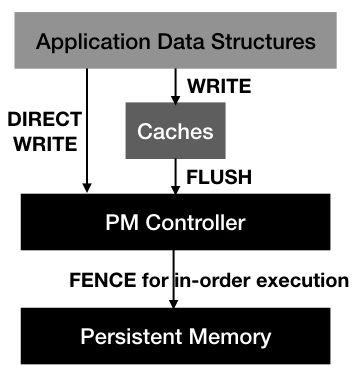
\includegraphics[width=\columnwidth]{figures/nvm-architecture.jpg}
    \caption{\emph{The architecture of Persitent Memory.}}
    \label{fig:architecture}
    \vspace{-0.3in}
\end{figure}


PM-CHECKER\footnote{https://github.com/SoujanyaPonnapalli/ASE-396-CourseProject}
models the architecture as shown in the Figure-\cite{fig-nvm-architecture}.

%\section{Desired Outcomes}


%\clearpage

% \nocite{*}
\bibliographystyle{is-unsrt}
%\bibliographystyle{ACM-Reference-Format}
\bibliography{ref}

\end{document}
